\section{Domæneanalyse}

\begin{figure}
\centering
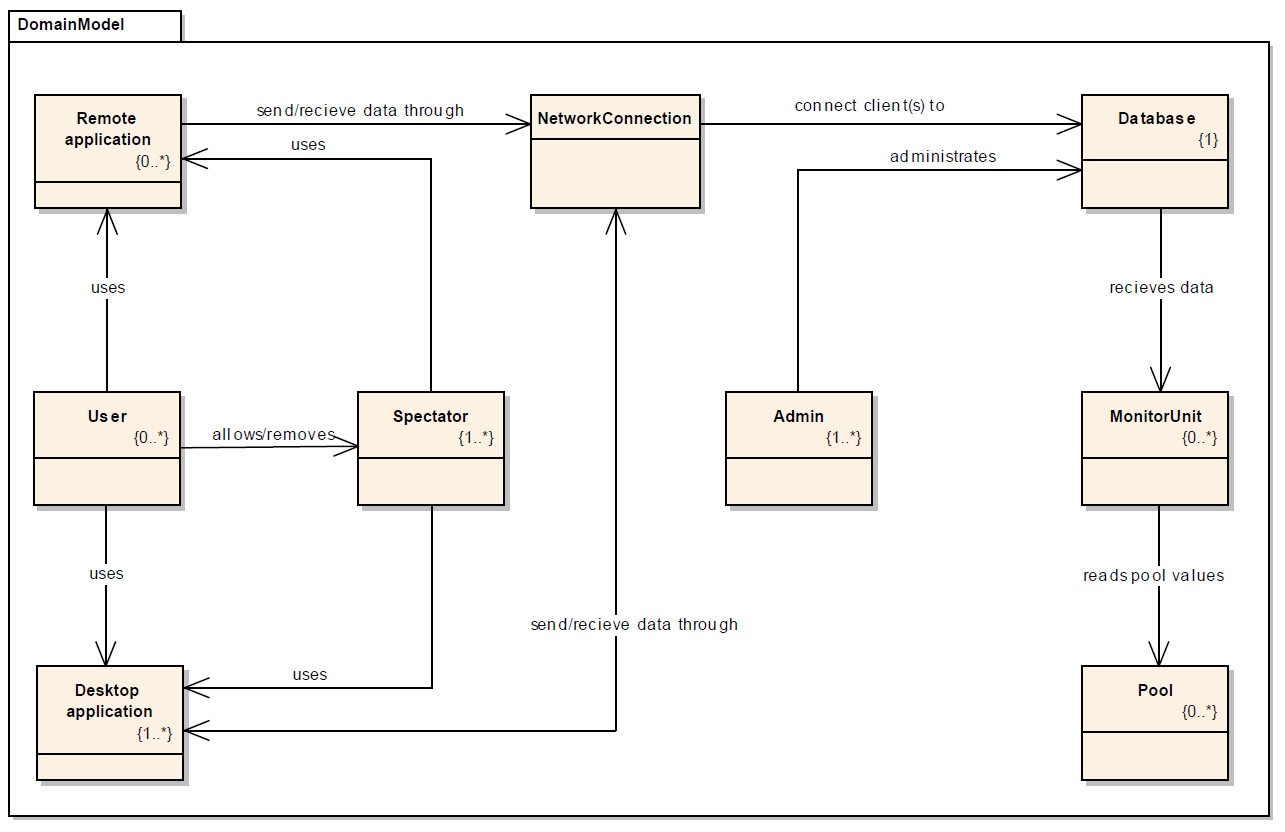
\includegraphics[width=\linewidth]{figs/domainModel}
\caption{Domænemodel for systemet}
\label{fig:domainModel}
\end{figure}

\subsection{Domænebeskrivelser}
Med udgangspunkt i modellen på figur~\ref{fig:domainModel} er der opstillet analyser af de enkelte domæner.

\subsubsection{User}
User er systemet primære bruger. En user kan tillade og/eller fjerne spectators. En user kan regulere pH/klor/temperatur værdier inden for evt. lovmæssige begrænsninger. Tilføjelse\footnote{Mulighed for tilføjelse af  MonitorUnits giver User mulighed for at tilføje flere/større pools og/eller MonitorUnits.} af MonitorUnits er brugerens ansvar. En User har mulighed for at sende en Spectate Invitation til en anden User. Dette gøres ved at sende et link\footnote{En User kan gennem Desktop applikationen få genereret et link som brugeren selv står for at sende.}  til anden partens email-addresse.

\subsubsection{Spectator}
En spectator er en User der med tillladelse fra en anden User får mulighed for at se med på dennes pooldata. Hvis den anden User har et system bestående af flere MonitorUnits.

\subsubsection{Desktop application}
Desktop applikationens primære formål er at gengive pooldata som findes på Databasen. En User kan igennem Desktop applikationen:

\begin{itemize}
	\item Logge ind med personlig brugerprofil.
	\item Generere et link til invitation af Spectator.
	\item Se grafisk gengivelse af historisk data.
	\item Se nuværende Pool data.
	\item Sætte target\footnote{  Ønskede værdier for pH, klor og varme.} værdier for Pool.
	\item Registrere en eller flere MonitorUnits.
\end{itemize}

\subsubsection{Remote application}
En Remote application er en “lightweight” udgave af Desktop applikationen. Denne applikations formål er at User kan danne sig et overblik over dataen fra de MonitorUnits der er tilknyttet konto.

\subsubsection{NetworkConnection}
Til at transmittere data fra MonitorUnit til Database, samt fra Database til Desktop applikation og Remote applikation benyttes en netværksforbindelse.  For at systemet skal fungere er det et krav at både Desktop og remote applikation, databaseserver samt MonitorUnit\footnote{  MonitorUnit har ikke en direkte forbindelse til internettet, men benytter sig af en endnu ikke defineret mediator.} har forbindelse til internettet.

\subsubsection{Admin}
En Admin er en “official” fra SmartPool\texttrademark, og har rettigheder til at fjerne brugere fra systemet. Det er Admins ansvar at de lovmæssige standarder for pH/klor/varme værdier er defineret i Databasen.

\subsubsection{Database}
Databasen indeholder brugerdata, såsom brugerens email-adresse, registrerede MonitorUnits, samt måledata. Måledata gemmes i en endnu udefineret tidsperiode, således at User har mulighed for at få en grafisk gengivelse\footnote{Evt. Graf, søjlediagram og lign.} af historisk data.

\subsubsection{MonitorUnit}
En MonitorUnit registreres hos SmartPool gennem Desktop applikationen. Med hver MonitorUnit medfølger et serienummer som bruges ved registrering. En MonitorUnit er enheden der måler pH, frit\footnote{Frit klor angriber bakterier, alger og svampeorganismer. Med tiden transformeres frit klor til bunden klor.} klor og total\footnote{Total klor er summen af frit klor og bunden klor.} klor samt varmeværdier i en Pool. Det er MonitorUnit der står for behandling\footnote{Da der er en sammenhæng~\ref{fig:chlorinePh} mellem målte pH-værdier og effektivitet af frit klor skal den rå data gennemgå en hidtil udefineret matematisk behandling for at kunne vise User relevant information.} af rå data. De rå data bruges til at beregne forholdet mellem bunden\footnote{Bunden klor er ineffektivt, lugter kraftigt og irriterer øjne og slimhinder.} klor og frit klor samt poolens overordnede sundhedskarakteristika. MonitorUnits ansvar er således:

\paragraph{Måling af data}
\begin{itemize}
	\item Måling af total klor.
	\item Måling frit klor.
	\item Måling af pH-værdi.
	\item Måling af Temperatur.
\end{itemize}

\paragraph{Behandling af rå data}
\begin{itemize}
	\item Beregning af bunden klor.
	\item Beregning af klor der bør tilføres/fjernes fra poolen.
	\item Beregning af den mængde syre/base der skal tilføres poolen.
\end{itemize}

\begin{figure}
\centering
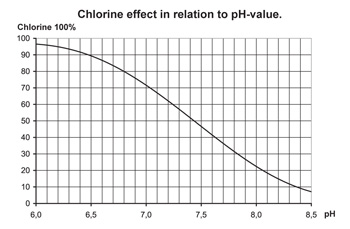
\includegraphics[width=0.6\linewidth]{figs/chlorinePh.png}
\caption{Sammenhæng mellem effektivitet af frit klor og pH værdi. Kilde: \url{http://www.pahlen.com/users-guide/ph-and-chlorine}}
\label{fig:chlorinePh}
\end{figure}


\subsubsection{Pool}
Pool er den enhed der males på. En pool kan være af hvilken som helst størrelse og form. Hver Pool kan associeres med en MonitorUnit